\section{Introduction}\label{sec:introduction}

The term Industry 4.0 (I. 4.0), as it was introduced by the German government in an effort to kick start a new paradigm in the manufacturing domain, describes a model towards enabling smart, flexible and predictive manufacturing, therefore optimising existing production processes and creating new business opportunities. \cite{i40gov} I. 4.0, also stated as the 4th Industrial Revolution\cite{revolution}, consists of four essential principles: interconnection between various devices (sensors, control units, machines, etc.) on the shop floor, information transparency to enable the creation of digital twins (virtual representations of objects), assistance for human operators and the use of Cyber-Physical-Systems (CPS) to enable smart manufacturing by applying decentralized decision making at the lower levels of production, therefore incorporating communication technologies, Internet of Things (IoT) and Machine Learning approaches. \cite{design}  

The implementation of the I. 4.0 concept is thus transforming the current automation pyramid \cite{autoPy} towards Smart Factories \cite{smartFac}, where not only the factories themselves, but where also the products are interconnected resulting in a decentralized/distributed ecosystem which is depicted in Fig. 1. The advantages of Smart Manufacturing over the traditional approach lie in the ability to analyse the running processes more efficiently as well as to apply reasoning to the data, which enables predictive manufacturing where machines can be controlled on a finer scale, resulting in individual maintenance scheduling on the shop floor and therefore in an improved production cycle.\cite{cpsAdv}

\begin{figure}
	\centering
	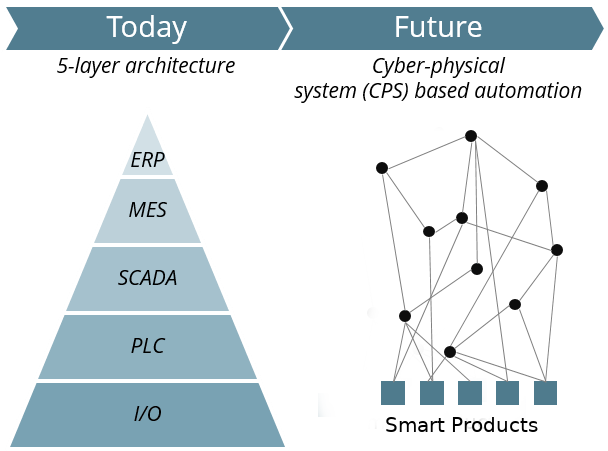
\includegraphics[scale=0.3]{comparison_autoHira_SF.png}
	\caption{Comparison between the traditional 5-layer automation Hierarchie and the future production architecture based on CPSs}
\end{figure}

However the implementation of the I.4.0 concept currently suffers from different drawbacks, as the manufacturing context applies different limitations on the integration. One of the key drawbacks lies in the latency requirements of factories. \cite{latency} Depending on the domain, it may be required to provide up to real time communication between devices as even small latencies can lead to delays of the production/assembly lines or even outages. Another problem arises from the amount of devices that gather data and therefore the amount of data that has to be processed. \cite{bigData} Even small devices can accumulate large sets of data over time, thus resulting in large datasets for the shop floor, as many thousand sensors and machines are part of the shop floor, and therefore requiring big data concepts. Given that most current implementations rely on a centralized cloud approach(a key enabler of automation), this creates a prominent data stream and therefore a heavy load towards the cloud, resulting in a bottleneck and leading to inefficient processing of the data. Another major concern is the power consumption of the sensing devices. \cite{fogDep} As sensing devices are usually constrainted and in certain use cases located in places difficult to reach efficiently, it is of importance to define communication methods that reduce the energy consumption of the devices, thus improving the battery lifetime.

Edge technologies introduce a way to tackle the above stated problems by improving the computational workflow. The term Edge refers to concepts where the processing of data is not achieved at a centralized node, but where the logic of the system is pushed to the edges of the network and thus closer to the devices. \cite{edgeDef} This concept is sometimes also referred to as FOG computing as these terms are not strictly defined and therefore used interchangeably. One way to differentiate these terms is depicted in Fig.2, where the Edge layer refers to the devices and the Fog layer represents a higher processing step. The addition of this processing step between the device layer and the cloud introduces a possibility to improve for example the latency of such systems.

\begin{figure}
	\centering
	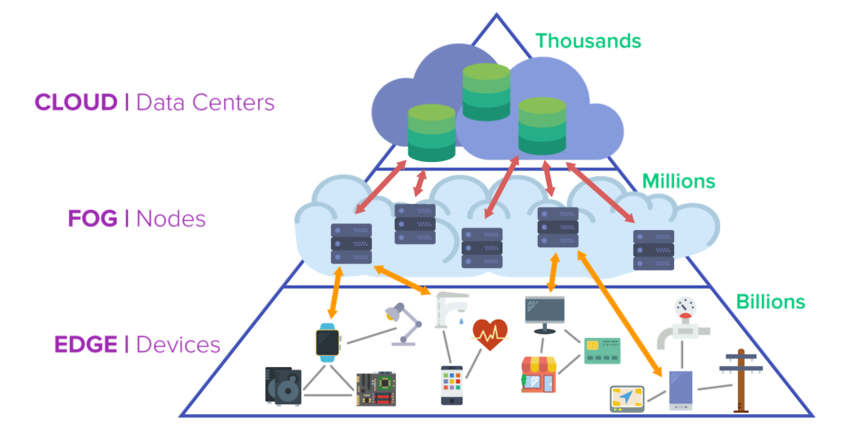
\includegraphics[scale=0.3]{edge_fog_cloud.png}
	\caption{Example of the division between Edge/Fog and the Cloud}
\end{figure}

This paper surveys the current trends in industrial edge computing, which leads towards smart manufacturing. It identifies key technologies, introduces concepts to integrate these technologies into existing production facilities as well as provides an overview on the benefits as well as drawbacks of these systems. This paper is therefore organized as follows. Section II provides an outline of related work on this topic. Section III introduces key technologies used for industrial edge computing, Section IV outlines integration concepts of these approaches and in Section V a discussion on the current state of industrial edge computing is provided. Section VI concludes this paper.